%%
% SigLog paper on HoTT
% May-December 2014
% IHP, CMU
%%
\documentclass[11pt]{article}
\usepackage{amsmath}
\usepackage{amssymb,latexsym}
\usepackage{amsthm}
\usepackage{bm}
\message{<Paul Taylor's Proof Trees, 2 August 1996>}
%% Build proof tree for Natural Deduction, Sequent Calculus, etc.
%% WITH SHORTENING OF PROOF RULES!
%% Paul Taylor, begun 10 Oct 1989
%% *** THIS IS ONLY A PRELIMINARY VERSION AND THINGS MAY CHANGE! ***
%%
%% 2 Aug 1996: fixed \mscount and \proofdotnumber
%%
%%      \prooftree
%%              hyp1            produces:
%%              hyp2
%%              hyp3            hyp1    hyp2    hyp3
%%      \justifies              -------------------- rulename
%%              concl                   concl
%%      \thickness=0.08em
%%      \shiftright 2em
%%      \using
%%              rulename
%%      \endprooftree
%%
%% where the hypotheses may be similar structures or just formulae.
%%
%% To get a vertical string of dots instead of the proof rule, do
%%
%%      \prooftree                      which produces:
%%              [hyp]
%%      \using                                  [hyp]
%%              name                              .
%%      \proofdotseparation=1.2ex                 .name
%%      \proofdotnumber=4                         .
%%      \leadsto                                  .
%%              concl                           concl
%%      \endprooftree
%%
%% Within a prooftree, \[ and \] may be used instead of \prooftree and
%% \endprooftree; this is not permitted at the outer level because it
%% conflicts with LaTeX. Also,
%%      \Justifies
%% produces a double line. In LaTeX you can use \begin{prooftree} and
%% \end{prootree} at the outer level (however this will not work for the inner
%% levels, but in any case why would you want to be so verbose?).
%%
%% All of of the keywords except \prooftree and \endprooftree are optional
%% and may appear in any order. They may also be combined in \newcommand's
%% eg "\def\Cut{\using\sf cut\thickness.08em\justifies}" with the abbreviation
%% "\prooftree hyp1 hyp2 \Cut \concl \endprooftree". This is recommended and
%% some standard abbreviations will be found at the end of this file.
%%
%% \thickness specifies the breadth of the rule in any units, although
%% font-relative units such as "ex" or "em" are preferable.
%% It may optionally be followed by "=".
%% \proofrulebreadth=.08em or \setlength\proofrulebreadth{.08em} may also be
%% used either in place of \thickness or globally; the default is 0.04em.
%% \proofdotseparation and \proofdotnumber control the size of the
%% string of dots
%%
%% If proof trees and formulae are mixed, some explicit spacing is needed,
%% but don't put anything to the left of the left-most (or the right of
%% the right-most) hypothesis, or put it in braces, because this will cause
%% the indentation to be lost.
%%
%% By default the conclusion is centered wrt the left-most and right-most
%% immediate hypotheses (not their proofs); \shiftright or \shiftleft moves
%% it relative to this position. (Not sure about this specification or how
%% it should affect spreading of proof tree.)
%
% global assignments to dimensions seem to have the effect of stretching
% diagrams horizontally.
%
%%==========================================================================

\def\introrule{{\cal I}}\def\elimrule{{\cal E}}%%
\def\andintro{\using{\land}\introrule\justifies}%%
\def\impelim{\using{\Rightarrow}\elimrule\justifies}%%
\def\allintro{\using{\forall}\introrule\justifies}%%
\def\allelim{\using{\forall}\elimrule\justifies}%%
\def\falseelim{\using{\bot}\elimrule\justifies}%%
\def\existsintro{\using{\exists}\introrule\justifies}%%

%% #1 is meant to be 1 or 2 for the first or second formula
\def\andelim#1{\using{\land}#1\elimrule\justifies}%%
\def\orintro#1{\using{\lor}#1\introrule\justifies}%%

%% #1 is meant to be a label corresponding to the discharged hypothesis/es
\def\impintro#1{\using{\Rightarrow}\introrule_{#1}\justifies}%%
\def\orelim#1{\using{\lor}\elimrule_{#1}\justifies}%%
\def\existselim#1{\using{\exists}\elimrule_{#1}\justifies}

%%==========================================================================

\newdimen\proofrulebreadth \proofrulebreadth=.05em
\newdimen\proofdotseparation \proofdotseparation=1.25ex
\newdimen\proofrulebaseline \proofrulebaseline=2ex
\newcount\proofdotnumber \proofdotnumber=3
\let\then\relax
\def\hfi{\hskip0pt plus.0001fil}
\mathchardef\squigto="3A3B
%
% flag where we are
\newif\ifinsideprooftree\insideprooftreefalse
\newif\ifonleftofproofrule\onleftofproofrulefalse
\newif\ifproofdots\proofdotsfalse
\newif\ifdoubleproof\doubleprooffalse
\let\wereinproofbit\relax
%
% dimensions and boxes of bits
\newdimen\shortenproofleft
\newdimen\shortenproofright
\newdimen\proofbelowshift
\newbox\proofabove
\newbox\proofbelow
\newbox\proofrulename
%
% miscellaneous commands for setting values
\def\shiftproofbelow{\let\next\relax\afterassignment\setshiftproofbelow\dimen0 }
\def\shiftproofbelowneg{\def\next{\multiply\dimen0 by-1 }%
\afterassignment\setshiftproofbelow\dimen0 }
\def\setshiftproofbelow{\next\proofbelowshift=\dimen0 }
\def\setproofrulebreadth{\proofrulebreadth}

%=============================================================================
\def\prooftree{% NESTED ZERO (\ifonleftofproofrule)
%
% first find out whether we're at the left-hand end of a proof rule
\ifnum  \lastpenalty=1
\then   \unpenalty
\else   \onleftofproofrulefalse
\fi
%
% some space on left (except if we're on left, and no infinity for outermost)
\ifonleftofproofrule
\else   \ifinsideprooftree
        \then   \hskip.5em plus1fil
        \fi
\fi
%
% begin our proof tree environment
\bgroup% NESTED ONE (\proofbelow, \proofrulename, \proofabove,
%               \shortenproofleft, \shortenproofright, \proofrulebreadth)
\setbox\proofbelow=\hbox{}\setbox\proofrulename=\hbox{}%
\let\justifies\proofover\let\leadsto\proofoverdots\let\Justifies\proofoverdbl
\let\using\proofusing\let\[\prooftree
\ifinsideprooftree\let\]\endprooftree\fi
\proofdotsfalse\doubleprooffalse
\let\thickness\setproofrulebreadth
\let\shiftright\shiftproofbelow \let\shift\shiftproofbelow
\let\shiftleft\shiftproofbelowneg
\let\ifwasinsideprooftree\ifinsideprooftree
\insideprooftreetrue
%
% now begin to set the top of the rule (definitions local to it)
\setbox\proofabove=\hbox\bgroup$\displaystyle % NESTED TWO
\let\wereinproofbit\prooftree
%
% these local variables will be copied out:
\shortenproofleft=0pt \shortenproofright=0pt \proofbelowshift=0pt
%
% flags to enable inner proof tree to detect if on left:
\onleftofproofruletrue\penalty1
}

%=============================================================================
% end whatever box and copy crucial values out of it
\def\eproofbit{% NESTED TWO
%
% various hacks applicable to hypothesis list 
\ifx    \wereinproofbit\prooftree
\then   \ifcase \lastpenalty
        \then   \shortenproofright=0pt  % 0: some other object, no indentation
        \or     \unpenalty\hfil         % 1: empty hypotheses, just glue
        \or     \unpenalty\unskip       % 2: just had a tree, remove glue
        \else   \shortenproofright=0pt  % eh?
        \fi
\fi
%
% pass out crucial values from scope
\global\dimen0=\shortenproofleft
\global\dimen1=\shortenproofright
\global\dimen2=\proofrulebreadth
\global\dimen3=\proofbelowshift
\global\dimen4=\proofdotseparation
\global\count255=\proofdotnumber
%
% end the box
$\egroup  % NESTED ONE
%
% restore the values
\shortenproofleft=\dimen0
\shortenproofright=\dimen1
\proofrulebreadth=\dimen2
\proofbelowshift=\dimen3
\proofdotseparation=\dimen4
\proofdotnumber=\count255
}

%=============================================================================
\def\proofover{% NESTED TWO
\eproofbit % NESTED ONE
\setbox\proofbelow=\hbox\bgroup % NESTED TWO
\let\wereinproofbit\proofover
$\displaystyle
}%
%
%=============================================================================
\def\proofoverdbl{% NESTED TWO
\eproofbit % NESTED ONE
\doubleprooftrue
\setbox\proofbelow=\hbox\bgroup % NESTED TWO
\let\wereinproofbit\proofoverdbl
$\displaystyle
}%
%
%=============================================================================
\def\proofoverdots{% NESTED TWO
\eproofbit % NESTED ONE
\proofdotstrue
\setbox\proofbelow=\hbox\bgroup % NESTED TWO
\let\wereinproofbit\proofoverdots
$\displaystyle
}%
%
%=============================================================================
\def\proofusing{% NESTED TWO
\eproofbit % NESTED ONE
\setbox\proofrulename=\hbox\bgroup % NESTED TWO
\let\wereinproofbit\proofusing
\kern0.3em$
}

%=============================================================================
\def\endprooftree{% NESTED TWO
\eproofbit % NESTED ONE
% \dimen0 =     length of proof rule
% \dimen1 =     indentation of conclusion wrt rule
% \dimen2 =     new \shortenproofleft, ie indentation of conclusion
% \dimen3 =     new \shortenproofright, ie
%                space on right of conclusion to end of tree
% \dimen4 =     space on right of conclusion below rule
  \dimen5 =0pt% spread of hypotheses
% \dimen6, \dimen7 = height & depth of rule
%
% length of rule needed by proof above
\dimen0=\wd\proofabove \advance\dimen0-\shortenproofleft
\advance\dimen0-\shortenproofright
%
% amount of spare space below
\dimen1=.5\dimen0 \advance\dimen1-.5\wd\proofbelow
\dimen4=\dimen1
\advance\dimen1\proofbelowshift \advance\dimen4-\proofbelowshift
%
% conclusion sticks out to left of immediate hypotheses
\ifdim  \dimen1<0pt
\then   \advance\shortenproofleft\dimen1
        \advance\dimen0-\dimen1
        \dimen1=0pt
%       now it sticks out to left of tree!
        \ifdim  \shortenproofleft<0pt
        \then   \setbox\proofabove=\hbox{%
                        \kern-\shortenproofleft\unhbox\proofabove}%
                \shortenproofleft=0pt
        \fi
\fi
%
% and to the right
\ifdim  \dimen4<0pt
\then   \advance\shortenproofright\dimen4
        \advance\dimen0-\dimen4
        \dimen4=0pt
\fi
%
% make sure enough space for label
\ifdim  \shortenproofright<\wd\proofrulename
\then   \shortenproofright=\wd\proofrulename
\fi
%
% calculate new indentations
\dimen2=\shortenproofleft \advance\dimen2 by\dimen1
\dimen3=\shortenproofright\advance\dimen3 by\dimen4
%
% make the rule or dots, with name attached
\ifproofdots
\then
        \dimen6=\shortenproofleft \advance\dimen6 .5\dimen0
        \setbox1=\vbox to\proofdotseparation{\vss\hbox{$\cdot$}\vss}%
        \setbox0=\hbox{%
                \advance\dimen6-.5\wd1
                \kern\dimen6
                $\vcenter to\proofdotnumber\proofdotseparation
                        {\leaders\box1\vfill}$%
                \unhbox\proofrulename}%
\else   \dimen6=\fontdimen22\the\textfont2 % height of maths axis
        \dimen7=\dimen6
        \advance\dimen6by.5\proofrulebreadth
        \advance\dimen7by-.5\proofrulebreadth
        \setbox0=\hbox{%
                \kern\shortenproofleft
                \ifdoubleproof
                \then   \hbox to\dimen0{%
                        $\mathsurround0pt\mathord=\mkern-6mu%
                        \cleaders\hbox{$\mkern-2mu=\mkern-2mu$}\hfill
                        \mkern-6mu\mathord=$}%
                \else   \vrule height\dimen6 depth-\dimen7 width\dimen0
                \fi
                \unhbox\proofrulename}%
        \ht0=\dimen6 \dp0=-\dimen7
\fi
%
% set up to centre outermost tree only
\let\doll\relax
\ifwasinsideprooftree
\then   \let\VBOX\vbox
\else   \ifmmode\else$\let\doll=$\fi
        \let\VBOX\vcenter
\fi
% this \vbox or \vcenter is the actual output:
\VBOX   {\baselineskip\proofrulebaseline \lineskip.2ex
        \expandafter\lineskiplimit\ifproofdots0ex\else-0.6ex\fi
        \hbox   spread\dimen5   {\hfi\unhbox\proofabove\hfi}%
        \hbox{\box0}%
        \hbox   {\kern\dimen2 \box\proofbelow}}\doll%
%
% pass new indentations out of scope
\global\dimen2=\dimen2
\global\dimen3=\dimen3
\egroup % NESTED ZERO
\ifonleftofproofrule
\then   \shortenproofleft=\dimen2
\fi
\shortenproofright=\dimen3
%
% some space on right and flag we've just made a tree
\onleftofproofrulefalse
\ifinsideprooftree
\then   \hskip.5em plus 1fil \penalty2
\fi
}

%==========================================================================
% IDEAS
% 1.    Specification of \shiftright and how to spread trees.
% 2.    Spacing command \m which causes 1em+1fil spacing, over-riding
%       exisiting space on sides of trees and not affecting the
%       detection of being on the left or right.
% 3.    Hack using \@currenvir to detect LaTeX environment; have to
%       use \aftergroup to pass \shortenproofleft/right out.
% 4.    (Pie in the sky) detect how much trees can be "tucked in"
% 5.    Discharged hypotheses (diagonal lines).

\usepackage[all,cmtip]{xy}
\input{diagxy}
\CompileMatrices       
\usepackage{url}
\usepackage{tikz}
\usepackage{pdfpages}

\usepackage[color=green!40]{todonotes}



% categories
\newcommand{\C}{\ensuremath{\mathbb{C}}}
\newcommand{\B}{\ensuremath{\mathbb{B}}}
\newcommand{\N}{\ensuremath{\mathbb{N}}}
\newcommand{\T}{\ensuremath{\mathbb{T}}}
\newcommand{\CC}{\ensuremath{\mathcal{C}}}
\newcommand{\BB}{\ensuremath{\mathcal{B}}}
%\newcommand{\EE}{\ensuremath{\mathcal{E}}}
\newcommand{\psh}[1]{\ensuremath{\mathsf{Set}^{#1^{\mathrm{op}}}}}
\newcommand{\Set}{\ensuremath{\mathsf{Set}}}
\newcommand{\Cat}{\ensuremath{\mathsf{Cat}}}
\newcommand{\covpsh}[1]{\ensuremath{\mathsf{Set}^{#1}}}
%\renewcommand{\to}{\ensuremath{\rightarrow}}
\newcommand{\pocorner}[1][dr]{\save*!/#1+1.2pc/#1:(1,-1)@^{|-}\restore}
\newcommand{\pbcorner}[1][dr]{\save*!/#1-1.2pc/#1:(-1,1)@^{|-}\restore}
\newcommand{\y}{\ensuremath{\mathsf{y}}} % Yoneda embedding

% arrows
\newcommand{\hook}{\ensuremath{\hookrightarrow}}
\newcommand{\mono}{\ensuremath{\rightarrowtail}}
%\newcommand{\epi}{\ensuremath{\twoheadrightarrow}}


% cubical sets
\newcommand{\I}{\ensuremath{\mathrm{I}}}
\renewcommand{\H}{\ensuremath{\mathbb{H}}}
\newcommand{\HH}{\ensuremath{\mathcal{H}}}

% type theory
\newcommand{\G}{\ensuremath{\Gamma}}
\newcommand{\defeq}{=_{\mathrm{def}}}
\newcommand{\type}{\mathsf{type}}       
\newcommand{\types}[2]{#1 \vdash #2:\type}
\newcommand{\Gtypes}[1]{\types{\Gamma}{#1}}
\newcommand{\term}[2]{#1\,:\,#2}
\newcommand{\terms}[2]{#1 \vdash #2}
\newcommand{\Gterms}[1]{\terms{\Gamma}{#1}}
\newcommand{\ext}[2]{{#1\!\centerdot\! #2}}
\newcommand{\ty}{\ensuremath{\,:\,}}
\newcommand{\pair}[1]{\ensuremath{\langle #1\rangle}}
\newcommand{\exdot}{\ensuremath{\!\centerdot\!}}
\newcommand{\texdot}{\ensuremath{\centerdot}}

% Id types
\newcommand{\Id}{\mathsf{Id}}
\newcommand{\id}[1]{\Id_{#1}}
\newcommand{\refl}{\mathsf{refl}}
\newcommand{\rec}{\mathsf{rec}}
\newcommand{\idrec}{\mathsf{idrec}}
\newcommand{\jay}{\mathsf{j}}
\renewcommand{\i}{\mathsf{i}}

% Universe
\newcommand{\U}{\ensuremath{\mathcal{U}}}
\newcommand{\UU}{\ensuremath{\widetilde{\mathcal{U}}}}

% theorem styles
\newtheorem{theorem}{Theorem}
\newtheorem*{theorem*}{Theorem}
\newtheorem{proposition}[theorem]{Proposition} 
\newtheorem{lemma}[theorem]{Lemma}
\newtheorem{corollary}[theorem]{Corollary} 

\theoremstyle{remark}
\newtheorem{remark}[theorem]{Remark} 
\newtheorem*{remarks*}{Remarks}
\newtheorem{example}[theorem]{Example}

\theoremstyle{definition}
\newtheorem{definition}[theorem]{Definition}

%%%%%%%%%%%%%%%%%%%%%%%%%%%%%%%%%%%%%%%%%%%%%%%%%%%%
\begin{document}
%%%%%%%%%%%%%%%%%%%%%%%%%%%%%%%%%%%%%%%%%%%%%%%%%%%%

\title{Homotopy Type Theory: Unified Foundations of Mathematics and Computation\thanks{ Thanks to Daniel Grayson,
    Michael Mislove, and Vladimir Voevodsky for helpful comments on an earlier draft.  Of course, the authors alone are
    still responsible for any errors or misstatements.}  } \author{Steve Awodey \and Robert Harper}
\date{\today}
\maketitle
%\todo[author=SA]{Note proposed new title.  I'm trying to avoid the term "Univalent foundations" here and throughout.}  

%%%%%%%%%%%%%%%%%%%%%%%%%%%%%%%%%%%%%%%%%%%%%%%%%%%%

%   \todo[inline,author=SA]{
%   
%    - "The biggest criticism overall from VV is that we do not represent the history fully and
%  faithfully," OK, I've made some revisions to that.
%  
%   - "that there are technical mistakes surrounding the use of the word ``proposition'' for other than a
%  $-1$-type, esp. LEM," fixed that where i could find it, but didn't find it much.
%  
%   - "and that we do not state clearly what problems are solved and what remain open." I don't see this either -- we do state some such.
%   
%  - "Because of his objections about the validity of HIT's, any statements involving them are, to him, conditional on their validity." this is not our problem.
%   
% - "He also objects to subjective statements about beauty." changed these. 
%   
% - "He feels that we've presented the subject as ``closed'' whereas there are lots of opportunities for more work. " see above. 
%     
%-  "And he feels that ``Univalent Framework'' is the right term to use for the foundational program he is pursuing that emphasizes machine-checked proof." He can write his own article to promote this term -- I don't feel obliged to use it.}
%

\noindent Homotopy type theory is a recently-developed unification of previously disparate frameworks, which can serve
to advance the project of formalizing and mechanizing mathematics.  One framework is based on a computational conception
of the type of a construction, the other is based on a homotopical conception of the homotopy type of a space.  
%Indeed,
%the name ``homotopy type theory'' can be read in two ways, as ``(homotopy type) theory'' and ``homotopy (type theory)'',
%neatly summarizing a consolidation of ideas lying at the heart of the subject.
The computational notion of type has its origins in Brouwer's program of intuitionism, which sought to ground
mathematics in the concept of an effective construction (one would say ``algorithm'' these days).  The homotopical
notion comes from Grothendieck's late conception of  homotopy types of spaces as represented by $\infty$-groupoids
\cite{GrothPS}.  The computational perspective was developed most fully by Per Martin-L\"{o}f, leading in particular to
his Intuitionistic Theory of Types~\cite{mltt}, on which the formal system of homotopy type theory is based.  The
connection to homotopy theory was first hinted at in the groupoid interpretation of Hofmann and
Streicher~\cite{HS,HofmannM:gromtt}.  It was then made explicit by several researchers, roughly
simultaneously.\footnote{%
  Awodey and Warren~\cite{AW} showed that the basic system of Martin-L\"{o}f type theory can be interpreted in a Quillen
  model category (an abstract framework for doing homotopy theory); Lumsdaine \cite{L} and van den Berg and Garner
  \cite{vandenBergB:typwg} showed that every type in the system has the structure of an $\omega$-category (a structure
  closely related to that of an $\infty$-groupoid); Gambino and Garner \cite{GG} showed that the type theory itself
  supports a weak factorization system (the basic building block of a Quillen model structure); and both Streicher
  \cite{StreicherNote} and Voevodsky \cite{VVnote} proposed interpretations into the category of simplicial sets, using
  ideas from homotopy theory.}  The connection was clinched by Voevodsky's introduction of the \emph{univalence axiom},
which is motivated by the homotopical interpretation, and which relates type equality to homotopy equivalence~\cite{KLV,APW}.

%\todo[inline,author=RH]{Based on
%  what I got from VV, here we should say that the idea of the homotopy interpretation was in the air already in 2006, as
%  evidenced by the abstracts at the Uppsala meeting on this topic, with significant contributions from Garner,
%  Streicher, Hyland, van den Berg, Gambino, Warren discussing the subject and problems such as the Beck Condition.  We
%  should cite the Uppsala abstracts and Streicher's unpublished notes that appear to be what he spoke about at the
%  meeting.  We should also cite VV's 2006 ``Homotopy Lambda Calculus'' manuscript as initial work on the subject, and,
%  as now, the Streicher-Hofmann groupoid model.  And then the AW paper and VV's Coq library as crucial initial steps.
%}
%Because univalence plays such a central role, Voevodsky has suggested that the unification of the computational and
%homotopical perspectives may be called the \emph{Univalent Framework} unifying two major lines of development in
%mathematics. 

% Sorry, but the following paragraph is really rough.  I'll try to polish it up.
%
%Since Brouwer, constructive foundations have often been misconstrued as incompatible with classical mathematics.  By
%contrast \emph{univalent foundations} as formulated in the framework of homotopy type theory here is fully compatible
%with classical mathematics, and indeed contains within it a classically inspired concept of a proposition as well as a
%concept of set that is compatible with both classical reasoning principles and such set existence principles as the
%axiom of choice.  The key to achieving this unification is to avoid postulating globally reasoning principles, such as
%the decidability of every type, that would be inconsistent with univalence, but which may be postulated locally, for
%example the decidability of every proposition in the aforementioned sense.  Remarkably, it is exactly these reasoning
%principles that are avoided in constructive foundations, opening the door to the unification of the constructive
%(computational) and homotopic (spatial) interpretations of types whose implications are only just beginning to be
%understood.

Constructive foundations are often regarded as incompatible with classical mathematics.  By
contrast, the framework of homotopy type theory is fully compatible with classical mathematics, and indeed allows for a classical conception of proposition, as well as a conception of set that is compatible with such principles as the axiom of choice.  
The key to achieving this unification is to avoid postulating generally certain reasoning principles, such as the decidability of every type, although these may still  be postulated ``locally", for example the decidability of every \emph{proposition}.  
It is notable that these same reasoning principles are also those that are usually avoided in constructive foundations, opening the door to the unification of the constructive (computational) and homotopic (spatial) interpretations of types, the implications of which are only just beginning to be understood.
Moreover, by not insisting on these principles globally, it is possible to consider a far richer notion of type than has
previously been considered in the computational approach, namely one in which types are abstract spaces that may have non-trivial
higher-dimensional structure, like the $n$-spheres for all $n\geq 0$.  In conventional foundations, such
as axiomatic set theory, these objects are presented as structured sets representing certain conceptions of space,
such as topological spaces.  Here, instead, such higher-dimensional objects arise ``synthetically''
in much the way that lines and triangles in Euclid's geometry are primitive abstract objects, rather than being comprised of analytic point-sets.  This provides a new perspective on some familiar constructions in homotopy theory, such as the homotopy groups of
a space~\cite{HoTTbook,LS-Circ,LB-PinSn} and the construction of so-called Eilenberg-MacLane spaces~\cite{LF-EM}, with specified
homotopy groups.  Moreover, new proofs of some standard results have a distinctively ``logical'' flavor, in combination with more ``geometric'' and
``topological'' elements.
% sorry, but the following remarks are completely mysterious at this point, before having introduced the connection between identity types and paths
%, arising from the way in which higher-dimensional spaces are represented using a so-called
%\emph{proof-relevant} notion of equality, called \emph{identifications}.

What is it that makes this new unification possible?  Although it may be too early to formulate a single, deep unifying
principle, it is possible to make a few observations that will give the reader a sense of its inevitability.  
First, all of the constructions of Intuitionistic Type Theory, including especially the previously enigmatic identity type, are
homotopy invariant, in the sense that type families and mappings between types inherently respect identifications
(paths, homotopies, or deformations).  Moreover, the formation of indexed products and sums of types, which correspond to analogous constructions on spaces, respect the homotopically motivated notion of equivelence of types,corresponding to the homotopy equivalence of spaces.  This invariance essentially follows from the basic fact that Martin-L\"{o}f's ingenious concept of the \emph{identity type} corresponds to the path space of a space, and since everything in the formal system respects identity, everything in the interpretation respects homotopy, which is determined by identfication along paths.
Second, a characteristic feature of both intuitionistic type theory and homotopy
theory is an emphasis on \emph{structure} over \emph{property}.  Under the propositions-as-types conception of
intuitionistic logic,\footnote{See, \textit{e.g.}, \cite{PAT} for a recent survey.} types express propositions, and objects of
the type are proofs of those propositions in the form of mathematical constructions that provide evidence for their
truth.  A similar emphasis can be discerned in abstract homotopy theory, in which, \textit{e.g.}, paths (homotopies) may be seen
as evidence for the ``identification" of two points, and similarly for paths between the corresponding values of two
functions.  Two points are not merely ``equal", as a property, but rather are identified by a (not necessarily unique)
deformation, construction, or procedure.  This approach extends to higher dimensions, in that one may speak of the
identifications of two (parallel) identifications, at all higher dimensions.  Such a structure of a hierarchy of
identifications via path connectedness is found in standard settings for homotopy theory such as simplicial sets,
cubical sets, and globular sets, all of which stress the role of cells as identifications.

%
%We thus see a natural harmony between the constructively motivated concept of \emph{proof relevance}, in which proofs
%are mathematical objects classified by a type,  (\textit{i.e.}, points in a space),
% and the homotopically motivated emphasis on
% structure over property.  
An important advantage resulting from proof relevance is that it naturally 
supports a comprehensive approach to mechanized mathematics in which computer systems, such as Coq~\cite{Coq}
and Agda~\cite{Agda}, can be used to verify the correctness of mathematical arguments, of either a classical, set-theoretic
form, or a constructive, type-theoretic form.  In either case the proof of a theorem constitutes a formal mathematical
object whose validity can be independently checked, avoiding the need to rely on the correctness of the proof checker
itself.  Once a proof has been obtained, others can not only verify its correctness by the usual means, but can also
submit the proof to another checker, to ensure that it is valid according to the rules of type theory. 
% what is this talking about? what assumptions? what does GO'del have to do with it?
% this is way too cryptic, and anyway distractingly off-topic.
% \footnote{Of
%  course, one may question the meaningfulness of type theory itself.  But as G\"{o}del demonstrated such assumptions are
%  unavoidable.}  
This approach to verification is fundamentally the same as that proposed by de Bruijn in the Automath
system~\cite{Automath}, albeit applied to a language with richer foundational commitments than were considered there.
It should be contrasted with the approach of systems such as NuPRL~\cite{NuPRL} or HOL~\cite{HOL,HOL-Light}, that rely
on a small trusted code base to ensure the validity of proofs.

The idea of identifications of points in a space along a continuous path, and of higher identifications of paths as homotopies, etc., leads to Voevodsky's conception of a hierarchy of \emph{homotopy levels}, or
\emph{h-levels} for short, which is definable within type theory.  Whereas the usual hierarchy of size is determined by type
universes or large cardinals in type theory or set theory, the hierarchy of h-levels is based instead on the internal
structure of types.  Roughly speaking, the lowest level consists of the types that have at most one element, up to
path-connectedness; these are called \emph{propositions}, and they correspond to the (empty or) contractible spaces.
The next level, called \emph{sets}, consists of those types whose identity types are themselves propositions --- two
elements of a set are ``equal in at most one way".  After that come the types whose
identity types are sets; these are the \emph{groupoids}.  And so on, with the types at level $n+1$ being those whose identity types have 
level $n$, for all $n\geq 0$.  Just the recognition that this hierarchy of h-levels is present in the system of all types
has been a huge advance in our understanding of type theory; previously, it was simply a mystery that some types were
fully determined by their elements, while others seemed to behave as though they had some further structure.  The
construction of quotient types, for example, is now greatly simplified when one knows that the equivalence relation
being factored out is a family of propositions, and not of ``higher-dimensional" types.  For another example, for types
$A$ and $B$ that are propositions, the relevant notion of equivalence is \emph{logical equivalence}, represented by the
type $A\leftrightarrow B$.  For sets, the relevant notion is \emph{isomorphism} $A\cong B$, and for groupoids, there is
the notion of \emph{(categorical) equivalence} $A\simeq B$.  Each of these concepts results by specializing the single,
uniform notion of \emph{equivalence of types} $A\simeq B$ (also due to Voevodsky) to the respective cases of
propositions, sets, and groupoids.

In this setting, Voevodsky's univalence axiom can be stated as the assertion that the type $A\simeq B$ of all
equivalences between two types $A$ and $B$ is itself equivalent to their identity type,
\[\tag{UA}
(A\simeq B)\ \simeq\  \id{}(A,B).
\]
Thus in particular, logically equivalent propositions will be identified, as in the original, extensional type theory of
Church \cite{Church}.  Isomorphic sets, too, will be identified ``up to homotopy'', \textit{i.e.}, by paths between them
in the universe of all types, and similarly for equivalent groupoids, and equivalent types in general.  Note that this
stipulation also serves to specify the otherwise underdetermined identity type $ \id{}(A,B)$.

This is not really the place for a systematic introduction (for that, see \cite{HoTTbook}), but a brief example may
serve to convey a bit of the flavor of the new approach, especially the distinctive intermingling of logical and
homotopical ideas.  As is the case in conventional Martin-L\"of type theory, the basic types of booleans $\B$ and
natural numbers $\N$ can have at most one identification between any two elements; that is, given say $n, m : \N$ and
$p,q: \id{\N}(n,m)$ in the identity type of $n$ and $m$, we always have some
$\alpha:\id{\left(\id{\N}(n,m)\right)}(p,q)$ identifying $p$ and $q$.  In this sense, there is no real information in
the type $\id{\N}(n,m)$, apart from whether or not it is inhabited.  Such types with at most one identification between
any two elements are called ``sets''.  Any types that can be constructed from $\B$, $\N$, or any other sets, by means of
the usual type constructors of dependent sum $\Sigma_{x:A}\,B(x)$ and dependent product $\Pi_{x:A}\,B(x)$ (which include
$A\times B$ and $A\rightarrow B$ as special cases) are also sets, and the same is true for the identity types
$\id{A}(a,a')$ for $a,a':A$, for any set~$A$.

An example of a type that is not a set is the circle (or ``$1$-sphere'') $S^1$, which has a base point $b: S^1$ and a
generating loop $ p :\id{S^1}(b,b)$.  There are then many different self-identifications, which may be labelled
$$\refl(b),\, p,\, p\cdot p,\, ... :\id{S^1}(b,b).$$ 
Here $\refl(b)$ is the trivial identification, \textit{i.e.}, the
canonical witness to the reflexivity of identity.  There is also the identification $p$, which is different from
$\refl(b)$ in the sense that $\id{\left(\id{S^1}(b,b)\right)}(\refl(b), p)$ is empty.  We can think of $p$ homotopically
as the continuous ``path" that goes once around the circle.

\begin{figure}\centering
  \begin{tikzpicture}[xscale=1,yscale=1]
     \draw[->] (0,-2) circle (1.4 and 1.4);
     \node (p) at (1.7,-2) {$p$};
     \node[fill,circle,inner sep=1pt,label={below:$b$}] at (0,-3.4) {};
  \end{tikzpicture}
\caption{The 1-sphere $S^1$}\label{fig:s1}
\end{figure}

By the (function witnessing the) transitivity of equality, 
\[
(-)\cdot(-) : \id{S^1}(a,b) \times \id{S^1}(b,c)\to \id{S^1}(a,c),
\]
 there are also the ``paths'' $p\cdot p,\, p\cdot p\cdot p,\, \ldots$.   And by symmetry,
 \[
 (-)^{-1}:\id{S^1}(a,b) \to \id{S^1}(b,a),
 \]
 there are similarly the paths $p^{-1},\, p^{-1}\cdot p^{-1}, \ldots :\id{S^1}(b,b)$.  Although $S^1$ is therefore not a set, it can be shown that $\id{S^1}(b,b)$ is one; that is, the types $\id{\left(\id{S^1}(b,b)\right)}(x,y)$ are either inhabited (by reflexivities) or empty, depending on whether or not $x=y$, for all $x,y : \id{S^1}(b,b)$.  Indeed, one can show that $\id{S^1}(b,b) \cong \mathbb{Z}$, \textit{i.e.}, the fundamental group of the type $S^1$ is the integers, as it should be (see \cite{LS-Circ} for the details).  
% In a situation like this, where the $\id{}$-type is always a set, we say that $S^1$ is a ``(homotopy) 1-type".  
The proof of this uses the univalence axiom, together with the specification of $S^1$ as a new kind of \emph{higher} inductive type, generalizing the usual inductive specification of the natural numbers and similar structures.  For $S^1$, the inductive specification essentially says that $S^1$ is ``the type freely generated by the base point $b:S^1$ and the loop $p:\id{S^1}(b,b)$", in the same sense that the usual inductive specification of $\N$ says that it is the type freely generated by $0:\N$ and the successor function $s:\N\to\N$.  
  
Another type that is not a set is the universe $\U$ of all (small) types.  According to the Univalence Axiom, identifications between types $A,B:\U$ correspond to equivalences $A\simeq B$, which as we said above are generalized type isomorphisms.  In fact, as already stated, if $A$ and $B$ themselves are sets, then an equivalence between them is just an isomorphism in the usual sense: a pair of maps back and forth that compose to the respective identity mapppings.  Now the booleans $\B$, for example, have two different isomorphisms $\B\cong \B$, namely the identity and the operation of ``negation'' $\neg:\B\to\B$, which swaps the truth values $0,1:\B$.  Thus by univalence there are two distinct identifications in $\id{\U}(\B,\B)$, corresponding to these distinct isomorphisms, and so $\U$ is not a set, but a ``higher-dimensional" type, like~$S^1$.  
 
Now observe that by the basic recursive property of $S^1$ as ``the type freely generated by a point with a loop on it'', there is a map $$\rec(\B,n): S^1 \to \U,$$ determined by sending the base point $b:S^1$ to the booleans $\B:\U$ and the generating loop $p : \id{S^1}(b,b)$ to (the loop corresponding under univalence to) negation, say $n : \id{\U}(\B,\B)$.  As a type of the form $S^1\to\U$, this $\rec(\B,n)$ is thus a family of types over $S^1$, sometimes called a ``dependent type" and written $$x:S^1 \vdash \rec(\B,n)(x).$$  Homotopically, such a type-family is interpreted as a ``fibration" $E\to S^1$, where the total space $E$ is just the sum type $\Sigma_{x:S^1}\,\rec(\B,n)(x)$, equipped with its usual indexing projection.  In the present case, the ``fiber" is then the type $\rec(\B,n)(b) = \B$, and the action on (elements of) $\B$ induced by the path $n: \id{S^1}(b,b)$ in the base is exactly the operation of negation $\neg : \B\to \B$.  Thus, from a homotopical point of view, we have constructed the ``twisted double cover'' of the circle (see Figure \ref{fig:winding}).
%
%\todo[inline]{fix this figure}
%
%\begin{figure}\centering
%  \begin{tikzpicture}[xscale=1.4,yscale=.6]
%    \node (R) at (2,1) {$S^1$};
%    \node (S1) at (2,-2) {$S^1$};
%    \draw[->] (R) -- node[auto] {$\mathsf{double}$} (S1);
%    \draw (0,-2) ellipse (1 and .4);
%    \draw[dotted] (1,0) arc (0:-30:1 and .8);
%    \draw (1,0) arc (0:90:1 and .8) arc (90:270:1 and .3) coordinate (t1);
%    \draw[white,line width=4pt] (t1) arc (-90:90:1 and .8);
%    \draw (t1) arc (-90:90:1 and .8) arc (90:270:1 and .3) coordinate (t2);
%    \draw[white,line width=4pt] (t2) arc (-90:90:1 and .8);
%    \draw (t2) arc (-90:90:1 and .8) arc (90:270:1 and .3) coordinate (t3);
%    \draw[white,line width=4pt] (t3) arc (-90:90:1 and .8);
%    \draw (t3) arc (-90:-30:1 and .8) coordinate (t4);
%    \draw[dotted] (t4) arc (-30:0:1 and .8);
%    \node[fill,circle,inner sep=1pt,label={below:\scriptsize $b$}] at (0,-2.4) {};
%    \node[fill,circle,inner sep=1pt,label={above left:\scriptsize 0}] at (0,.2) {};
%    \node[fill,circle,inner sep=1pt,label={above left:\scriptsize 1}] at (0,1.2) {};
%    \node[fill,circle,inner sep=1pt,label={above left:\scriptsize 2}] at (0,2.2) {};
%  \end{tikzpicture}
%  \caption{The twisted double cover of $S^1$ in classical topology}\label{fig:winding}
%\end{figure}
%
\begin{figure}\centering
  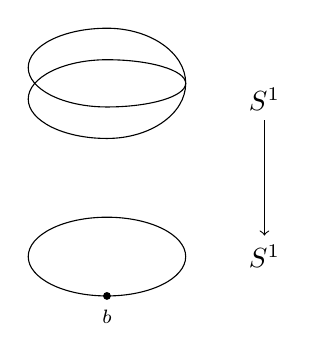
\begin{tikzpicture}[xscale=1,yscale=1]
    \node (R) at (2,0) {$S^1$};
    \node (S1) at (2,-2) {$S^1$};
    \draw[->] (R) -- node[auto] {} (S1);
    \draw (0,-2) ellipse (1 and .5);
%    \draw[dotted] (1,0) arc (0:-30:1 and .8);
%    \draw (0,5) arc (0:90:1 and .5) arc (90:270:1 and .5) coordinate (t1);
%    \draw (t1) arc (-90:45:1 and .5) ;% arc (90:270:1 and .3) coordinate (t2);
    \draw (-1,0) arc (180:270:1 and .5) coordinate (t1);
%    \draw[white,line width=4pt] (t1) arc (-90:90:1 and .8);
    \draw (t1) arc (-90:90:1 and .7) arc (90:270:1 and .5) coordinate (t2);
%    \draw[white,line width=4pt] (t2) arc (-90:90:1 and .8);
    \draw (t2) arc (-90:90:1 and .3) arc (90:180:1 and .5) coordinate (t3);
%    \draw[white,line width=4pt] (t3) arc (-90:90:1 and .8);
 %  \draw (t3) arc (-90:-30:1 and .8) coordinate (t4);
 %   \draw[dotted] (t4) arc (-30:0:1 and .8);
    \node[fill,circle,inner sep=1pt,label={below:\scriptsize $b$}] at (0,-2.5) {};
%    \node[fill,circle,inner sep=1pt,label={above left:\scriptsize 0}] at (0,.2) {};
%    \node[fill,circle,inner sep=1pt,label={above left:\scriptsize 1}] at (0,1.2) {};
%    \node[fill,circle,inner sep=1pt,label={above left:\scriptsize 2}] at (0,2.2) {};
  \end{tikzpicture}
  \caption{The twisted double cover of $S^1$}\label{fig:winding}
\end{figure}
%
This construction from homotopy theory is closely related to the celebrated Hopf fibration which, among other things, can be used to compute some of the higher homotopy groups of the spheres $S^2$ and $S^3$.  Indeed, one can construct the Hopf fibration in homotopy type theory in much the same way as the foregoing example, using univalence, negation, winding around the circle, and other constructions derived from combinations of logical, type-theoretic, and homotopical ideas (see \cite{HoTTbook}, \S 8.5). 

% This sort of reasoning gives an entirely new ``synthetic" approach to some areas of classical mathematics like algebraic topology, which not only allows for the explicit logical formalization of classical results like the calculations of homotopy groups of spheres, but also permits their formal verification in computational proof systems based on a constructive system of logic.

%%%%%%%%%%%%
%
% the following bit expands on some of the material in 107-129, but also conflicts with it in some places 
% (e.g. "n-type" vs. "h-level").
% I have tried below to revise to avoid some repetition and make it more consistent, but this is just a suggestion.
% I am leaving the original here in comments for comparison and possible reuse.
%
%%%%%%%%%%%%
%
%An important point about univalent foundations is that it subsumes the classical set-theoretic framework for doing
%mathematics.  The hierarchy of $n$-types neatly accounts for classical set-theoretic foundations within a broader
%framework of homotopy types.  Specifically, $-1$-types, which have at most one element up to higher identification,
%correspond to classical proof-irrelevant propositions, except that whether to insist that every proposition be inhabited
%or empty remains a consistent choice that one may accept or reject at will.  The $0$-types, for which equality is a
%classical proposition ($-1$-type) that is taken to be ``self-evident'' or ``proof-irrelevant'' correspond to classical
%sets, without prior commitment to choice principles or whether membership is a boolean proposition; these can be taken
%as axioms according to preference, without fear of inconsistency.  The advantage of univalent foundations is that
%besides the familiar concepts of proposition (classically formalized as predicate calculus) and set (classically given
%by the Zermelo-Fr\"{a}nkel axioms), it provides an infinite hierarchy of dimensions extending beyond just these two.
%For example, the $1$-types are the natural setting for set-theoretic structures, such as groups or rings, that one may
%wish to identify up to isomorphism.  Because two groups, say, can be isomorphic in different ways, the evidence for
%their identification must provide the mutually inverse pairs of homomorpisms that constitute the identification.
%
%Another import aspect of univalent foundations is that it extends Martin-L\"{o}f's type theory~\cite{mltt} with an
%infinite hierarchy of dimensions that were hitherto inaccessible within the theory, even though models were known that
%exhibited higher-dimensional structure~\cite{HS}.  Type theory was conceived as a foundation for
%constructive mathematics, in which all constructions, including proofs of propositions, have direct computational
%meaning in accordance with Brouwer's original program.  This connection with computation has proved enormously
%influential in computer science, in particular in the theory of programming languages and the foundations of mechanized
%proof.  At present homotopy type theory exploits the concept of proof relevance that is central to the constructivist
%program (indeed, according to that program propositions are not just $-1$-types, but can be any $n$-type), and draws on
%the emphasis on abstract types (for example, in the treatment of the identification type as an abstraction in itself,
%rather than being encoded in terms of a concrete conception of homotopy).  The grand challenge is to extend the
%computational interpretation to the full hierarchy of $n$-types, providing a computational meaning for, say, mappings
%among higher-dimensional structures such as the spheres and toruses of arbitrary dimension.  Recent advances, such as
%the development of a constructively valid model using cubical sets~\cite{BCH}, strongly suggest that such a unification
%is possible in the near future.  The implications for computer science are only beginning to be
%explored~\cite{patch-theory}.
%
%It is a curious fact, made all the more interesting by the above-mentioned developments, that two of the most successful
%systems for mechanized proof, NuPRL~\cite{nuprl-book} and Coq~\cite{Coq}, are based on constructive type theory.  Why
%ought that be the case?  Univalent foundations seems to provide a clue, namely the importance of proof-relevance for
%both classical homotopy theory and constructive mathematics.  A significant contribution of homotopy type theory is that
%it exploits the axiomatic freedom of constructive mathematics (that is, the diminished emphasis on axioms that are
%inconsistent, at full strength, with univalence) to achieve a synthetic formulation of homotopy theory that is wholly
%coherent with constructive mathematics.  As Voevodsky has emphasized, classical theorem provers may only be used by
%rather involved encodings of the natural concept of space using structures such as topological spaces or simplicial
%sets, greatly impeding the process of formalization required to admit machine-checked proof.  This experiene parallels
%the development of high-level (abstract) programming languages that provide a synthetic concept of computation, rather
%than one based on low-level machine models such as the Turing machine or Random-Access Machine.  Thus we find that
%whether we are discussing mechanized proof or verified programming, Church's $\lambda$-calculus emerges as a central
%concept.  Perhaps this explains why constructive mathematics and mechanized proof are so tightly linked.
%

%\todo[author=RH]{revision looks good to me, but for one query below}

We can now say in a bit more detail how the univalent framework of homotopy type theory subsumes and extends the
classical, set-theoretic framework for doing mathematics, by making use of the hierarchy of h-levels, which includes
sets within a broader framework of homotopy types.  At the bottom level, the propositions (the types having at most one
element, up to higher identification) correspond to conventional, proof-irrelevant propositions; whether we also assert
the law of excluded middle in the form that every such proposition is either inhabited or empty is a further, consistent
assumption that may be made if classical logic is desired.  Next, the sets (for which equality is a proposition that is
taken to be ``self-evident'' or ``proof-irrelevant'') correspond to the usual sets, but now without any commitment to
choice principles, or whether membership is a boolean proposition.  Those further principles can still be consistently
taken as axioms if needed, but they are not required, even with the introduction of infinite sets such as the type of
natural numbers. Voevodsky's new insight, which plays such an important role in homotopy type theory, is that, besides
the familiar concepts of proposition (classically formalized in predicate calculus) and set (classically given by the
Zermelo-Fraenkel axioms), there is an infinite hierarchy of further dimensions extending beyond just these two.  The
groupoids (the next h-level above the sets), such as our example $S^1$, are the natural setting for systems of
set-theoretic structures, such as groups and rings, that one may wish to regard as identified up to isomorphism.
Because two groups, say, can be isomorphic in many different ways, however, the evidence for an identification is not a
trivial proposition, but consists in the mutually inverse pair of homomorpisms, \textit{i.e.}, the isomorphism, that
warrant it.  Here we see explicitly how proof-relevance (from constructivism) and the ``property-structure" distinction (from homotopy theory) coincide.

In this way we can now distinguish, within Martin-L\"{o}f type theory, an infinite hierarchy of different ``homotopical
dimensions" that were not fully recognized previously, despite such models as Hofmann and Streicher's two-dimensional
groupoid interpretation~\cite{HS} that strongly hinted at the importance of higher dimensions of structure.  Type theory
was, of course, originally conceived as a foundation for constructive mathematics, in which all constructions, including
proofs of propositions, have direct computational meaning in accordance with Brouwer's original program.  This
fundamental connection with computation has proved enormously influential in computer science, in particular in the
theory of programming languages and the foundations of mechanized proof.  Homotopy type theory makes essential use of the
concept of proof relevance, which is so central to the constructive program, and emphasizes a notion of abstract types that is
familiar from the theory of programming languages (\textit{e.g.}, the identity type is itself an abstraction, rather than being encoded in terms of a concrete definition of homotopy).  The grand challenge as of this writing is to
extend the computational interpretation to the univalence axiom, and therewith to the full hierarchy of h-levels, providing a computational meaning for, say, mappings among higher-dimensional structures such as the spheres and toruses of arbitrary dimension.  Recent advances,
such as the landmark development of a constructively valid model using cubical sets~\cite{BCH}, strongly suggest that
such a unification will be achieved in the near future.  The potential implications for computer science are only
beginning to be explored~\cite{AMLH}.

Perhaps the most important application of the unification of classical and constructive mathematics is the possibility
of applying systems of mechanized proof verification to broad swaths of classical mathematics that were previously
formalizable only via elaborate coding into set theory, and only in systems based on classical logic, which generally
lack the benefits resulting from the computational interpretation of constructive systems (\textit{e.g.}, the generation
of independently verifiable proof certificates).  The direct formalization of everything from quotient sets to
cohomology simplifies and streamlines the formalization of even advanced mathematics, and has the potential to
eventually make formal verification into a practical tool for the everyday mathematician.  Interestingly, this practical
development makes the logical foundations of mathematics finally relevant to the actual practice of mathematics, rather
than being just a theoretical possibility.  The result may be a new ``post-G\"odel" attitude toward foundations; for
when their only interest was theoretical, the phenomenon of incompleteness seemed to lessen the importance of logical
foundations in principle.  But with the actual practical benefits of formalization (increased rigor and certainty, ease
of remote collaboration, accumulation of results), the theoretical incompleteness phenomenon diminishes in importance,
and logical foundations can become a useful addition to the toolbox of the working mathematician.\footnote{See the code
  section of \url{http://homotopytypetheory.org}for links to shared repositories of mechanized mathematics in homotopy
  type theory using the Coq and Agda systems.}

%\todo[author=RH]{Not sure the preceding belongs here, but could perhaps by merged into what follows, and moved earlier
 % to the discussion of UF, of which mechanization is central.}

It is a curious fact, made all the more interesting by the above-mentioned developments, that two of the most successful
systems for mechanized proof, NuPRL~\cite{NuPRL} and Coq~\cite{Coq}, are both based on constructive type theory.  Why
ought that be the case?  Homotopy type theory may provide a clue in the importance of proof-relevance, and the
associated distinction between property and structure, in both constructive mathematics and homotopy theory.  The
univalent approach of homotopy type theory exploits the axiomatic freedom provided by constructive mathematics, allowing
it to rely far less on elaborate encodings which impede the process of formalization required to admit machine-checked
proof.  This experience parallels the development of high-level (abstract) programming languages that provide a
synthetic concept of computation, rather than one based on low-level machine models such as the Turing machine or
Random-Access Machine.  Thus we find that whether we are discussing mechanized mathematical proof or verified computer
programming, Church's $\lambda$-calculus emerges as a central concept.  Perhaps this explains why constructive
mathematics and mechanized proof are so tightly linked.  That they should also be entwined with homotopy theory --- one
of the most abstract, geometrical, and rarified areas of modern mathematics --- is an intriguing and challenging fact
inviting further investigation.


%%% Steve: Your citations below are intact.

% %%%%%%%%%%%%%%%%%%%%%%%%%%%%%%%%%%%%%%%%%%%%%%%%%%%%
% \begin{thebibliography}{300}
% %%%%%%%%%%%%%%%%%%%%%%%%%%%%%%%%%%%%%%%%%%%%%%%%%%%%

% \bibitem{AW}
% S.~Awodey and M.A.~Warren. Homotopy theoretic models of identity types. \emph{Math. Proc. Camb. Phil. Soc.}, 146, 45--55, 2009.

% \bibitem{GvdB}
% B.~van den Berg and R.~Garner. Topological and Simplicial Models of Identity Types. \emph{ACM Transactions on Computational Logic}, 13:1, 2012.

% \bibitem{CwF} 
% P.~Dybjer. ``Internal Type Theory." \emph{LNCS} 1158, 120--134, 1996.

% \bibitem{HS}
% M.~Hofmann and T.~Streicher.

% \bibitem{HoTTbook} 
% \emph{Homotopy Type Theory: Univalent Foundations of Mathematics}, The Univalent Foundations Program, Institute for Advanced Study, 2013. {\tt http://homotopytypetheory.org/book}

% \bibitem{KLV}  
% C.~Kapulkin, P.~LeFanu Lumsdaine and V.~Voevodsky, The Simplicial Model of Univalent Foundations. \emph{In preparation}, 2013.

% %

% \end{thebibliography}

\bibliographystyle{plain}
\bibliography{siglog}

%%%%%%%%%%%%%%%%%%%%%%%%%%%%%%%%%%%%%%%%%%%%%%%%%%%%
\end{document}
%%%%%%%%%%%%%%%%%%%%%%%%%%%%%%%%%%%%%%%%%%%%%%%%%%%%
